\documentclass[11pt]{article}
\usepackage[margin=2.5cm]{geometry}
\usepackage{amsmath,amssymb,bm}
\usepackage{graphicx}
\usepackage{booktabs}
\usepackage{array}
\usepackage{algorithm}
\usepackage{algpseudocode}
\usepackage{listings}
\usepackage{xcolor}
\usepackage[colorlinks=true,linkcolor=blue!50!black,urlcolor=blue!50!black]{hyperref}

\lstset{language=Python, basicstyle=\ttfamily\small, keywordstyle=\color{blue!70!black},
  commentstyle=\color{green!40!black}, stringstyle=\color{red!60!black},
  frame=single, columns=fixed, basewidth=0.5em, keepspaces=true, breaklines=true,
  escapeinside={(*@}{@*)}}

\newcommand{\R}{\mathbb{R}}
\newcommand{\xref}{x_{\mathrm{ref}}}

\title{Nonlinear Model-Predictive Control with CasADi:\\ the Cart-Pole Swing-Up}
\author{NOMICC 2026 --- self-study notes}
\date{}

\begin{document}
\maketitle

\begin{abstract}
We formulate the swing-up and stabilization of an inverted pendulum on a cart as a
nonlinear model-predictive control (NMPC) problem, discretize it by direct multiple
shooting, and solve the resulting sequence of nonlinear programs (NLPs) with CasADi
and the solvers Ipopt, Uno and CasADi's own SQP method.
The companion script is \texttt{nmpc\_cartpole.py}; every equation below is tagged
with the function that implements it.
\end{abstract}

\section{The model}\label{sec:model}

The cart (mass $M$) moves on a horizontal track; a pole of length $l$ with a point
mass $m$ at its tip is hinged to the cart. The state and control are
\[
  x = (p,\ \theta,\ v,\ \omega)^T \in \R^4, \qquad u = F \in \R,
\]
where $p$ is the cart position, $\theta$ the pole angle measured from the
\emph{downward} vertical ($\theta=0$ hanging, $\theta=\pi$ upright), $v=\dot p$,
$\omega=\dot\theta$, and $F$ the horizontal force on the cart. Lagrangian mechanics gives
\begin{equation}\label{eq:ode}
  \dot x = f(x,u) =
  \begin{pmatrix}
    v \\ \omega \\[2pt]
    \dfrac{F + m \sin\theta\,(l\omega^2 + g\cos\theta)}{M + m\sin^2\theta} \\[10pt]
    \dfrac{-F\cos\theta - m l \omega^2 \cos\theta\sin\theta - (M+m) g \sin\theta}{l\,(M + m\sin^2\theta)}
  \end{pmatrix}
\end{equation}
with $M=1$\,kg, $m=0.2$\,kg, $l=0.5$\,m, $g=9.81$\,m/s$^2$
(\texttt{cartpole\_ode}). The upright equilibrium $\xref=(0,\pi,0,0)$ is unstable,
and the system is underactuated (one input, two degrees of freedom), so the controller
has to ``pump'' energy into the pole before it can catch it.

\section{The optimal control problem}

Given the measured state $\hat x$ at time $t$, NMPC solves the finite-horizon problem
\begin{equation}\label{eq:ocp-cont}
\begin{aligned}
  \min_{x(\cdot),\,u(\cdot)} \quad & \int_0^{T} \ell\big(x(\tau),u(\tau)\big)\,d\tau + V_f\big(x(T)\big)\\
  \text{s.t.}\quad & \dot x(\tau) = f\big(x(\tau),u(\tau)\big),\quad x(0)=\hat x,\\
                   & |u(\tau)| \le F_{\max},\quad |p(\tau)| \le p_{\max},
\end{aligned}
\end{equation}
applies the first part of the optimal input, and repeats at the next sample.
We use the quadratic stage and terminal costs
\begin{subequations}\label{eq:costs}
\begin{align}
  \ell(x,u) &= \|x-\xref\|_Q^2 + R\,u^2, \label{eq:stage-cost}\\
  V_f(x)    &= \|x-\xref\|_P^2,           \label{eq:terminal-cost}
\end{align}
\end{subequations}
where $\|e\|_Q^2 = e^TQe$, with $Q=\mathrm{diag}(10,10,0.1,0.1)$, $R=0.01$, $P=10\,Q$, $F_{\max}=20$\,N,
$p_{\max}=1.5$\,m.

\section{Discretization: direct multiple shooting}

Choose a sampling time $\Delta t=0.05$\,s, a horizon of $N=40$ samples ($T=2$\,s),
and piecewise-constant controls $u(\tau)=u_k$ on $[k\Delta t,(k+1)\Delta t)$.
Let $\Phi(x,u)$ be the state after one sample, approximated by two explicit
Runge--Kutta-4 steps of length $h=\Delta t/2$ (\texttt{rk4\_step}). One RK4 step
maps $x$ to $x^+$ by
\begin{subequations}\label{eq:rk4}
\begin{align}
  k_1 &= f(x,u),\quad k_2 = f(x+\tfrac h2 k_1,u),\quad k_3 = f(x+\tfrac h2 k_2,u),\quad k_4=f(x+hk_3,u), \label{eq:rk4-stages}\\
  x^+ &= x + \tfrac h6 (k_1+2k_2+2k_3+k_4), \label{eq:rk4-update}
\end{align}
\end{subequations}
and $\Phi(x,u)$ applies this step twice.
In \emph{multiple shooting} the states at the sampling instants are kept as
optimization variables and the dynamics become equality (``continuity'' or ``gap'')
constraints. The NLP is (\texttt{build\_ocp})
\begin{subequations}\label{eq:nlp}
\begin{align}
  \min_{\substack{x_0,\dots,x_N\\ u_0,\dots,u_{N-1}}}\quad & J = \sum_{k=0}^{N-1} \Big(\|x_k-\xref\|_Q^2 + R u_k^2\Big) + \|x_N-\xref\|_P^2 \label{eq:nlp-obj}\\
  \text{s.t.}\quad & x_0 = \hat x, \label{eq:nlp-init}\\
  & x_{k+1} = \Phi(x_k,u_k), && k=0,\dots,N-1, \label{eq:nlp-dyn}\\
  & {-F_{\max}}\le u_k \le F_{\max}, && k=0,\dots,N-1, \label{eq:nlp-u}\\
  & {-p_{\max}}\le p_k \le p_{\max}, && k=1,\dots,N. \label{eq:nlp-p}
\end{align}
\end{subequations}
The objective \eqref{eq:nlp-obj} is the sum of the stage costs \eqref{eq:stage-cost} and
the terminal cost \eqref{eq:terminal-cost}; \eqref{eq:nlp-dyn} are the continuity
constraints.
The track bound is not imposed at $k=0$: $p_0=\hat p$ is data, not a decision, and
a (noisy) measurement just outside the track would otherwise make \eqref{eq:nlp}
infeasible.
A solver sees all unknowns stacked into one vector,
\[
  w = (x_0,u_0,x_1,u_1,\dots,x_{N-1},u_{N-1},x_N)\in\R^{5N+4},
\]
so \eqref{eq:nlp} is an NLP $\min_w F(w)$ s.t.\ $G(w)=0$, $w_L\le w\le w_U$.
For $N=40$ this has $204$ variables and $164$ equality constraints.

Figure~\ref{fig:ms} illustrates the idea on a coarse grid ($N=10$, $\Delta t=0.2$\,s),
writing $s_k$ for the shooting nodes $x_k$. Each node starts its own short integration,
and the solver is free to place the nodes anywhere. The initial guess may therefore have
gaps, and the continuity constraints close them only at the solution.

\begin{figure}[ht]
\centering
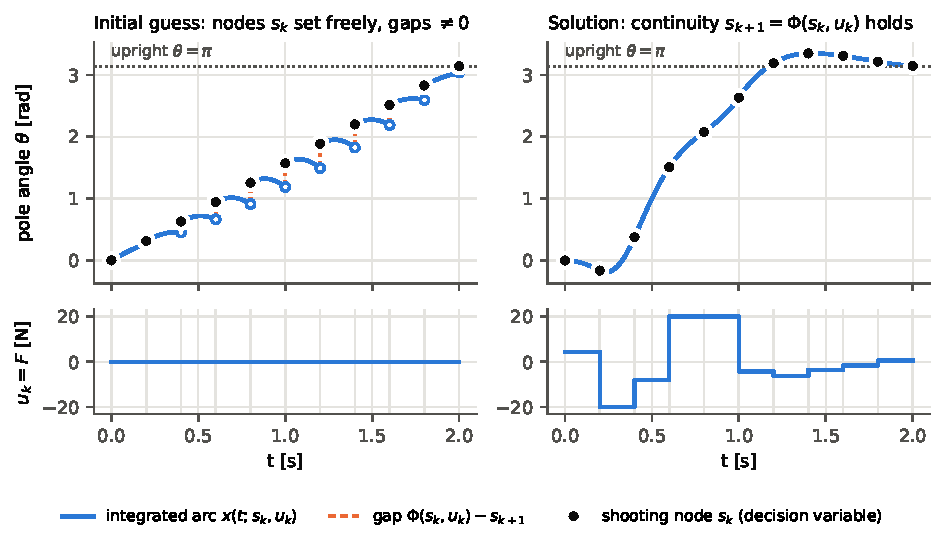
\includegraphics[width=\textwidth]{figures/multiple_shooting.pdf}
\caption{Direct multiple shooting for the cart-pole (only $\theta$ shown). \emph{Left:}
initial guess, with nodes $s_k$ on a straight line from hanging to upright and $u_k=0$.
Integrating the ODE from each node over one interval (blue arcs) does not reach the next
node, and the dashed gaps $\Phi(s_k,u_k)-s_{k+1}$ are the violated continuity constraints.
\emph{Right:} the NLP solution, where all gaps are closed, so the arcs join into one
trajectory of the ODE. The force is piecewise constant (bottom).}
\label{fig:ms}
\end{figure}

\paragraph{Why multiple rather than single shooting?}
Single shooting eliminates $x_1,\dots,x_N$ by forward simulation, leaving only
$u_0,\dots,u_{N-1}$. This gives a smaller but much more nonlinear problem: for an
unstable system the map $u\mapsto x_N$ is very sensitive, so Newton steps are poor.
Multiple shooting
(i) spreads the nonlinearity over many small, local constraints,
(ii) lets us initialize the state trajectory directly (for example with the previous
solution, or an infeasible guess), and
(iii) keeps the KKT matrix sparse and block-banded, which is what interior-point and
SQP solvers exploit.

\section{The receding-horizon loop}

NMPC turns the open-loop optimal control problem into a feedback law by re-solving it at
every sample (Figure~\ref{fig:nmpc}). At time $t_j$ it measures the state $\hat x_j$,
solves \eqref{eq:nlp} over the horizon $[t_j, t_j+T]$, applies only the first control
$u^\star_0$ for one sample, and discards the rest of the plan. At $t_{j+1}=t_j+\Delta t$ it
measures again and solves over the horizon shifted by one sample. The horizon ``recedes''
in front of the system, which gives the method its name.

\begin{figure}[ht]
\centering
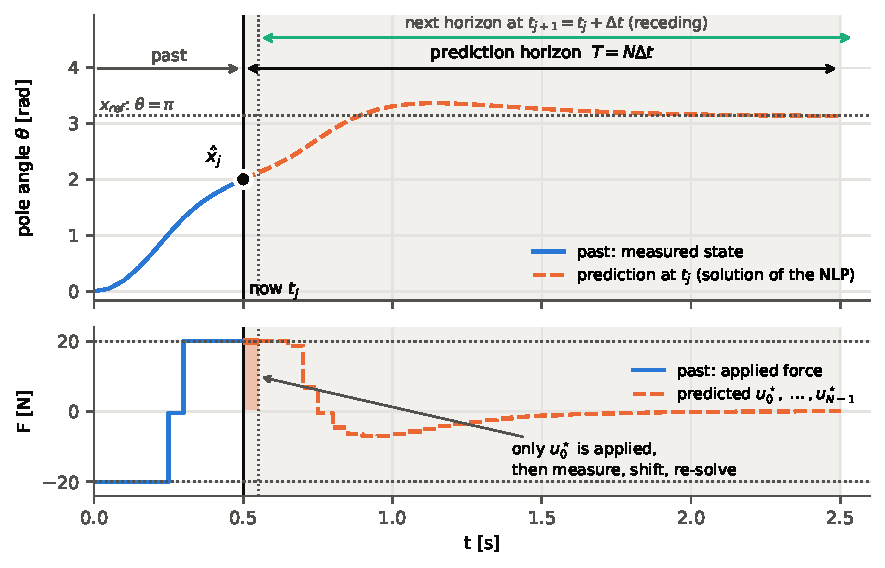
\includegraphics[width=0.9\textwidth]{figures/nmpc_principle.pdf}
\caption{The NMPC principle, at sample $j=10$ ($t_j=0.5$\,s) of the cart-pole swing-up.
To the left of ``now'' is the past (measured state and applied force). The shaded region
is the prediction horizon, with the predicted trajectory and control sequence from the
NLP solved at $t_j$. Only $u^\star_0$ (filled bar) is sent to the plant, and the whole
problem is solved again on the next horizon starting at $t_{j+1}$.}
\label{fig:nmpc}
\end{figure}

\begin{algorithm}[ht]
\caption{NMPC with shift warm start (\texttt{run\_closed\_loop})}
\begin{algorithmic}[1]
\State $x^{\mathrm{pl}}_0 \gets (0,0,0,0)$ \Comment{true plant state: hanging at rest}
\State initial guess $w^{(0)}$: $x_k=x^{\mathrm{pl}}_0$, $u_k=0$
\For{$j = 0,1,2,\dots$}
  \State measure $\hat x_j = x^{\mathrm{pl}}_j + \eta_j$, \ $\eta_j\sim\mathcal N(0,\sigma^2 I)$ \Comment{$\sigma=0$ by default}
  \State solve NLP \eqref{eq:nlp} with $x_0=\hat x_j$ from the guess $w^{(j)}$; obtain $w^\star_j$
  \State apply $u_j := u^\star_0$: $x^{\mathrm{pl}}_{j+1} = \Phi^{\mathrm{pl}}(x^{\mathrm{pl}}_j,u_j)$ \Comment{CVODES, true plant}
  \State $w^{(j+1)} \gets$ shift$(w^\star_j)$: $(x^\star_1,\dots,x^\star_N,x^\star_N;\ u^\star_1,\dots,u^\star_{N-1},u^\star_{N-1})$
\EndFor
\end{algorithmic}
\end{algorithm}

\paragraph{Warm starting.} Consecutive NLPs differ only in $\hat x$, so the shifted
solution is an excellent guess and the solver usually needs only a few iterations.

\paragraph{Plant vs.\ model.} In control, the \emph{plant} is the real physical system,
and the \emph{model} is the controller's mathematical approximation of it, used to
predict the future inside the NLP. In the script both are simulated, but they are
deliberately kept apart:

\begin{center}
\begin{tabular}{>{\raggedright\arraybackslash}p{0.17\textwidth}>{\raggedright\arraybackslash}p{0.36\textwidth}>{\raggedright\arraybackslash}p{0.36\textwidth}}
\toprule
 & \textbf{model} (inside the NLP) & \textbf{plant} (the ``real'' cart-pole) \\
\midrule
role & predicts $x_1,\dots,x_N$ through $x_{k+1}=\Phi(x_k,u_k)$
     & produces the next true state after $u_0$ is applied \\
integration & $\Phi$: fixed-step RK4, 2 substeps (\texttt{rk4\_step})
            & $\Phi^{\mathrm{pl}}$: adaptive CVODES, tight tolerances (\texttt{plant}) \\
pole mass & $m=0.2$\,kg & $0.2$\,kg; $0.26$\,kg with \texttt{--mismatch} \\
measurement & --- & $\hat x = x^{\mathrm{pl}} + \eta$, with \texttt{--noise} $\sigma$ \\
\bottomrule
\end{tabular}
\end{center}

\noindent Three kinds of discrepancy can be switched on:
\begin{enumerate}
\item \emph{Discretization error} (always present): RK4 with $h=0.025$\,s is accurate,
  so prediction and reality agree closely, and even the open-loop plan would nearly work.
\item \emph{Parametric model error} (\texttt{--mismatch}): the controller plans with the
  wrong pole mass, so the measured state after one sample differs from the predicted
  $x^\star_1$. Executing the first plan open loop would miss the upright position.
  Re-solving from the measured state at every sample (\emph{feedback}) corrects the error.
\item \emph{Measurement noise} (\texttt{--noise}~$\sigma$): the controller sees
  $\hat x_j = x^{\mathrm{pl}}_j + \eta_j$ with independent Gaussian noise of standard
  deviation $\sigma$ in every component (m, rad, m/s, rad/s), and treats it as exact.
  Each NLP is therefore solved for a slightly wrong initial state. The pole stays
  balanced but jitters, and the solver needs more iterations because the shifted guess
  is less accurate.
\end{enumerate}
The setup is still idealized: the full state is measured and there are no external
disturbances. A real implementation estimates $\hat x$ from noisy partial measurements
with a state estimator (an extended Kalman filter or moving-horizon estimation), which
itself solves an optimization problem much like \eqref{eq:nlp}, backwards in time.

\section{The CasADi code in one page}

The listing below is complete and runs as is. It builds the model \eqref{eq:ode}, the
RK4 map \eqref{eq:rk4}, and the NLP \eqref{eq:nlp}, and solves the first MPC problem.
The comment at the end of each line names the equation it implements.
\texttt{nmpc\_cartpole.py} contains the same code, split into functions.

\begin{lstlisting}
import casadi as ca
import numpy as np

# parameters
M, m, l, g = 1.0, 0.2, 0.5, 9.81           # cart, pole mass, length, gravity
N, dt = 40, 0.05                           # horizon N, sampling time Delta t
F_max, p_max = 20.0, 1.5                   # bounds in (*@(\ref{eq:nlp-u}), (\ref{eq:nlp-p})@*)
x_ref = ca.DM([0, np.pi, 0, 0])            # upright equilibrium
Q, R = ca.diag([10, 10, 0.1, 0.1]), 0.01   # weights in (*@(\ref{eq:stage-cost})@*)
P = 10 * Q                                 # weight in (*@(\ref{eq:terminal-cost})@*)

# the model xdot = f(x, u)
x = ca.SX.sym("x", 4)                      # x = (p, theta, v, omega)
u = ca.SX.sym("u")                         # u = F
th, v, om = x[1], x[2], x[3]
s, c = ca.sin(th), ca.cos(th)
den = M + m * s**2
xdot = ca.vertcat(v, om,                   # (*@(\ref{eq:ode})@*), rows 1-2
    (u + m * s * (l * om**2 + g * c)) / den,               # (*@(\ref{eq:ode})@*), row 3
    (-u * c - m * l * om**2 * c * s - (M + m) * g * s) / (l * den))  # (*@(\ref{eq:ode})@*), row 4
f = ca.Function("f", [x, u], [xdot])       # f(x, u) in (*@(\ref{eq:ode})@*)

# Phi(x, u): two RK4 steps of length h = dt/2
h = dt / 2
xk = x
for _ in range(2):
    k1 = f(xk, u)                          # (*@(\ref{eq:rk4-stages})@*)
    k2 = f(xk + h / 2 * k1, u)             # (*@(\ref{eq:rk4-stages})@*)
    k3 = f(xk + h / 2 * k2, u)             # (*@(\ref{eq:rk4-stages})@*)
    k4 = f(xk + h * k3, u)                 # (*@(\ref{eq:rk4-stages})@*)
    xk = xk + h / 6 * (k1 + 2 * k2 + 2 * k3 + k4)          # (*@(\ref{eq:rk4-update})@*)
Phi = ca.Function("Phi", [x, u], [xk])     # Phi in (*@(\ref{eq:nlp-dyn})@*)

# the NLP
opti = ca.Opti()
X = opti.variable(4, N + 1)                # x_0, ..., x_N
U = opti.variable(1, N)                    # u_0, ..., u_{N-1}
x0 = opti.parameter(4)                     # measured state xhat
J = 0
for k in range(N):
    e = X[:, k] - x_ref
    J += ca.bilin(Q, e, e) + R * U[:, k]**2                # stage cost (*@(\ref{eq:stage-cost})@*)
    opti.subject_to(X[:, k + 1] == Phi(X[:, k], U[:, k]))  # (*@(\ref{eq:nlp-dyn})@*)
eN = X[:, N] - x_ref
J += ca.bilin(P, eN, eN)                   # terminal cost (*@(\ref{eq:terminal-cost})@*)
opti.minimize(J)                           # (*@(\ref{eq:nlp-obj})@*)
opti.subject_to(X[:, 0] == x0)             # (*@(\ref{eq:nlp-init})@*)
opti.subject_to(opti.bounded(-F_max, U, F_max))            # (*@(\ref{eq:nlp-u})@*)
opti.subject_to(opti.bounded(-p_max, X[0, 1:], p_max))     # (*@(\ref{eq:nlp-p})@*), k = 1..N
opti.solver("ipopt")                       # or "uno", "sqpmethod", ...

# one MPC step (Algorithm 1, lines 4-6), from the hanging rest state
xhat = np.zeros(4)                         # measured state
opti.set_value(x0, xhat)
opti.set_initial(X, np.tile(xhat, (N + 1, 1)).T)           # guess w^(0): x_k = xhat
opti.set_initial(U, 0)                     # guess w^(0): u_k = 0
sol = opti.solve()
u_apply = sol.value(U)[0]                  # u_0^*, the only control sent to the plant
\end{lstlisting}
\texttt{Opti} collects the variables into $w$, the constraints
\eqref{eq:nlp-init}--\eqref{eq:nlp-p} into $g(w)$ with bounds, and passes \[
  \{\texttt{x}: w,\ \texttt{f}: J,\ \texttt{g}: g(w),\ \texttt{p}: \hat x\}
\]
to \texttt{nlpsol}. CasADi generates the exact gradient, constraint Jacobian and
Lagrangian Hessian by algorithmic differentiation, so no derivative is written by hand.

\section{Solvers}

All solvers below are bundled with the \texttt{casadi} pip wheel.
\begin{itemize}
\item \textbf{Ipopt}: primal-dual interior point method with filter line search. It is
  robust from poor starting points. Warm starting an interior point method is limited,
  because the barrier parameter pushes iterates away from active bounds.
\item \textbf{Uno} (\texttt{preset=ipopt}): Uno's reimplementation of an Ipopt-like
  interior point method.
\item \textbf{Uno} (\texttt{preset=filtersqp}): trust-region SQP with a filter
  (the \textsc{filterSQP} strategy); the QPs are solved by BQPD with active-set warm
  starts. Because an active-set SQP re-uses the previous active set, it is very
  effective in the warm-started MPC loop.
\item \textbf{sqpmethod}: CasADi's line-search SQP; its QP solver \texttt{qrqp} needs a
  convex QP, so we convexify the Lagrangian Hessian (\texttt{convexify\_strategy=eigen-clip}).
\end{itemize}

\begin{table}[ht]
\centering
\caption{Closed loop, $N=40$, 100 MPC steps, shift warm start (one run on a laptop;
your timings will differ).}\label{tab:solvers}
\begin{tabular}{lrrr}
\toprule
solver & 1st solve (cold) & mean iters, steps 2--100 & total iterations \\
\midrule
Ipopt                    & 60 & 5.3 & 581 \\
Uno, preset \texttt{ipopt}     & 64 & 5.4 & 596 \\
Uno, preset \texttt{filtersqp} & 21 & 1.4 & 155 \\
sqpmethod + qrqp         & 59 & 1.5 & 204 \\
\bottomrule
\end{tabular}
\end{table}

\section{Results}

Figure~\ref{fig:closed-loop} shows the closed loop: the controller first pushes the cart
to the left at full force, reverses to swing the pole up, saturates again, and catches
the pole within about one second. The track bound $|p|\le 1.5$ is approached but never
violated, and the force saturates at $\pm F_{\max}$ during the swing-up.

\begin{figure}[ht]
\centering
\IfFileExists{cartpole_closed_loop.png}{%
  \includegraphics[width=0.75\textwidth]{cartpole_closed_loop.png}}{%
  \fbox{\parbox{0.7\textwidth}{\centering Run \texttt{python nmpc\_cartpole.py --plot}
  to generate \texttt{cartpole\_closed\_loop.png}.}}}
\caption{Closed-loop states and force for the default settings.}\label{fig:closed-loop}
\end{figure}

\section{Remarks: nonconvexity and local solutions}

Problem \eqref{eq:nlp} is nonconvex (the dynamics are trigonometric equalities). The
solvers return \emph{local} solutions, and which local solution is found depends on the
initial guess. A striking example in this problem: with \texttt{--no-warmstart}, each NLP
is started from ``stay where you are with zero force''. The first solve still finds the
swing-up, but later cold-started solves converge to a different local minimizer that
keeps the pole hanging, so the closed loop never swings up. Warm starting
is part of the controller, not only a speed-up: it keeps successive solutions on the same
``branch''.

\section{Outlook}

Replacing $|F|\le F_{\max}$ by an on/off actuator $F\in\{-F_{\max},0,F_{\max}\}$ turns
\eqref{eq:nlp} into a mixed-integer NLP (MINLP), which can be solved with
\texttt{bonmin} (bundled with CasADi) or CAMINO. Contact or friction effects lead to
complementarity constraints (MPCC). These are the themes of the summer school.

\end{document}
